\section{Introduction}

\subsection{Background}
Everyone knows the best way to make a wish: picking up a dandelion in its iconic "puffball" stage, and blowing on it to release thousands of seeds into the environment. But, how much do these many seeds actually contribute to the growth and spread of dandelions? In this paper, we develop a mathematical model to predict the spread of dandelions across a plot of land and evaluate whether plants like dandelions are truly invasive.

Beginning as a "puffball," there are several phases that a dandelion progresses through in its lifetime. The first phase is when the seeds of a "puffball" spread, usually by wind. Once landed in soil, the seed will begin its plant phase, which has two main processes: (1) germination, where the seed breaks dormancy, and (2) growth as a plant, where the seed continues to adapt to the environment, eventually becoming the iconic bright yellow flower. Finally, in the third phase, the dandeolion flower returns to a puffball stage to disperse even more seeds, thereby restarting the cycle. In total, this cycle takes about 50 days to complete, and often resets for each individual plant due to predator consumption, inclement weather, or a possibly unsuccessful growth stage (Canadian Journal!!!).

\subsubsection{Phase 1: Seed}
In order for a seed to grow, certain environmental conditions must be met. In the event that conditions are not met, seeds often enter a dormant stage where they can remain beneath the earth until environmental conditions are met. Unlike most plants, the dandelion seed cannot lay dormant for long due to the high likelihood of premature consumption \cite{noauthor_dandelion_nodate-2}. Only around 2-4\% of seeds make it past the initial dispersal stage, the remainder of which is consumed by predators \cite{noauthor_dandelion_nodate-2}. Of the small amount that do survive, they typically germinate right away and survive until the next season \cite{noauthor_dandelion_nodate-2}.

\subsubsection{Phase 2: Plant}
In order for the seed to germinate, take root, and become a flowering plant, the seed must experience certain environmental conditions, such as the right temperature, light, and nutrients in the soil. The seed then grows until it enters its flowering stage, where the dandelion continues its growth process until it has transitioned into its puffball stage. 

\subsubsection{Phase 3: Puffball}
After flowering, the dandelion grows for around 10 days \cite{noauthor_dandelion_nodate-2}. After this period of growth, the dandelion enters a puffball stage. The puffball stage occurs when the seed-head of the plant fully emerges, replacing the distinctive yellow flowers, in order to disperse the seeds. The seed-head is a globe-shaped ball of seeds attached a long stem known as a pappus. The seeds connect to one another to form the seed-head until the right gust of wind comes and scatters the seeds off to take root in a new area.

\subsubsection{Death}
As a perennial plant, the taproot of the dandelion allows the plant to keep its roots for another year while the flowers and stem wither away in the winter. In the event of any damage to the portion of the plant above ground, the taproot remains rooted, and so, the dandelion continues to survive \cite{}. In order for a dandelion to fully die, either the taproot is removed from the ground or the plant reaches its life expectancy of 10-13 years (CITE!!!).

In Figure~\ref{fig:dandelionlifecycle}, we summarize the life-cycle of a dandelion (from seed through growth), from which we draw inspiration in our dandelion spread model.

\begin{figure}[h!]
\centering
    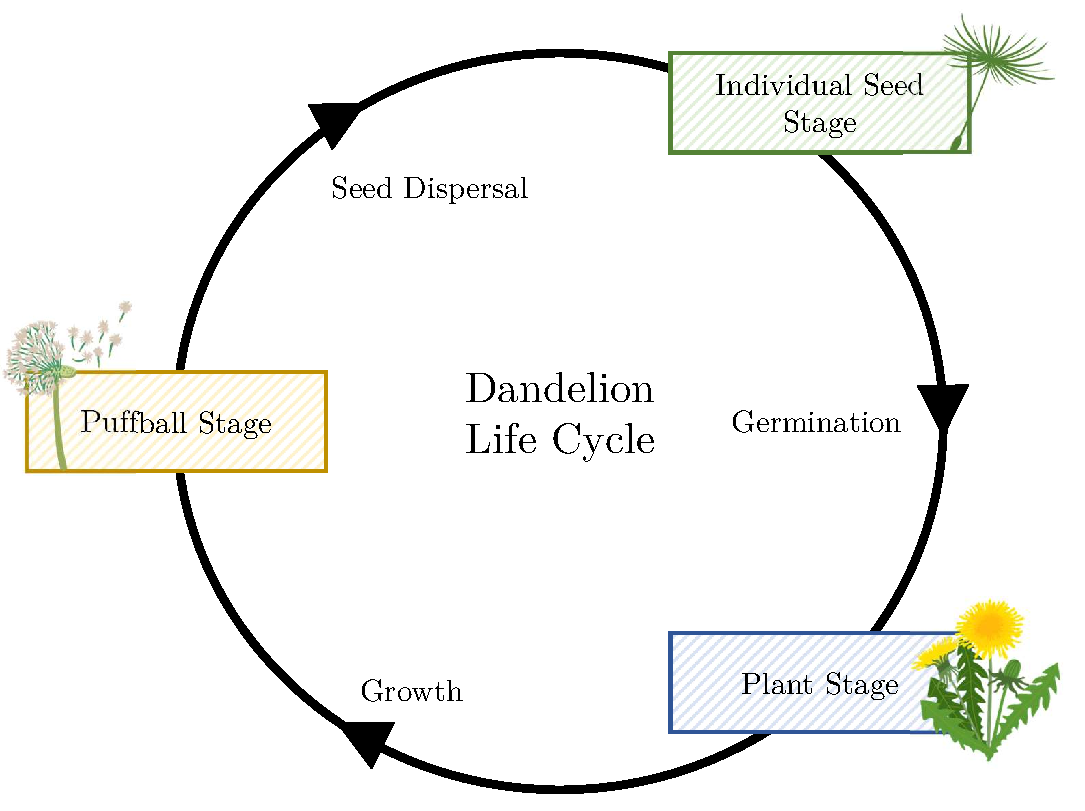
\includegraphics[scale=0.5]{figures/dandelionlifecycle.pdf}
    \captionsetup{width=0.9\textwidth}
    \caption{\textbf{Dandelion life-cycle.} A recurring process from a seed to germination to growth, then the dispersal of seeds again.}
    \label{fig:dandelionlifecycle}
\end{figure}

\subsection{Problem Restatement}

 \begin{enumerate}
 \item Develop a model to represent the spread of dandelions over the course of 1, 2, 3, 
6, and 12 months, given the model begins with a single dandelion in its puffball stage adjacent to an open, one-hectare plot of land.
\item Formulate a mathematical model capable of determining an ‘impact factor’ for invasive species.
\subitem a. Compute an impact factor for dandelions to test the model
\subitem b. Determine the impact factor for two other plant species of 
our choice that are often considered invasive.

\end{enumerate}
